%%%%%%%%%%%%%%%%%%%%%%%%%%%%%%%%%%%%%%%%%
% a0poster Portrait Poster
% LaTeX Template
% Version 1.0 (22/06/13)
%
% The a0poster class was created by:
% Gerlinde Kettl and Matthias Weiser (tex@kettl.de)
% 
% This template has been downloaded from:
% http://www.LaTeXTemplates.com
%
% License:
% CC BY-NC-SA 3.0 (http://creativecommons.org/licenses/by-nc-sa/3.0/)
%
%%%%%%%%%%%%%%%%%%%%%%%%%%%%%%%%%%%%%%%%%

%----------------------------------------------------------------------------------------
%	PACKAGES AND OTHER DOCUMENT CONFIGURATIONS
%----------------------------------------------------------------------------------------

\documentclass[a0,portrait]{a0poster}

\usepackage{multicol} % This is so we can have multiple columns of text side-by-side
\columnsep=100pt % This is the amount of white space between the columns in the poster
\columnseprule=3pt % This is the thickness of the black line between the columns in the poster

\usepackage[svgnames]{xcolor} % Specify colors by their 'svgnames', for a full list of all colors available see here: http://www.latextemplates.com/svgnames-colors
\usepackage{relsize}

\usepackage{times} % Use the times font
%\usepackage{palatino} % Uncomment to use the Palatino font
\usepackage{url}
\usepackage{graphicx} % Required for including images
\graphicspath{{figures/}} % Location of the graphics files
\usepackage{booktabs} % Top and bottom rules for table
\usepackage[font=small,labelfont=bf]{caption} % Required for specifying captions to tables and figures
\usepackage[]{algorithm2e}
\usepackage{amsfonts, amsmath, amsthm, amssymb} % For math fonts, symbols and environments
\usepackage{wrapfig} % Allows wrapping text around tables and figures
\usepackage{subfigure}

\begin{document}
%To scale up the font size of whole document
\relscale{1.62}

%----------------------------------------------------------------------------------------
%	POSTER HEADER 
%----------------------------------------------------------------------------------------

% The header is divided into two boxes:
% The first is 75% wide and houses the title, subtitle, names, university/organization and contact information
% The second is 25% wide and houses a logo for your university/organization or a photo of you
% The widths of these boxes can be easily edited to accommodate your content as you see fit

\begin{minipage}[b]{0.71\linewidth}
\VeryHuge \color{Black} \textbf{Optimizing Short Read Error Correction \\on Graphics Processing Unit (GPU)} \color{Black}\\[0.4cm] % Title
\huge Aman Mangal (amanmangal@gatech.edu) \\ Chirag Jain (cjain@gatech.edu)\\[0.5cm] % Author(s)
\huge Georgia Institute of Technology, Atlanta, GA\\ % University/organization
\end{minipage}
%
\begin{minipage}[b]{0.25\linewidth}
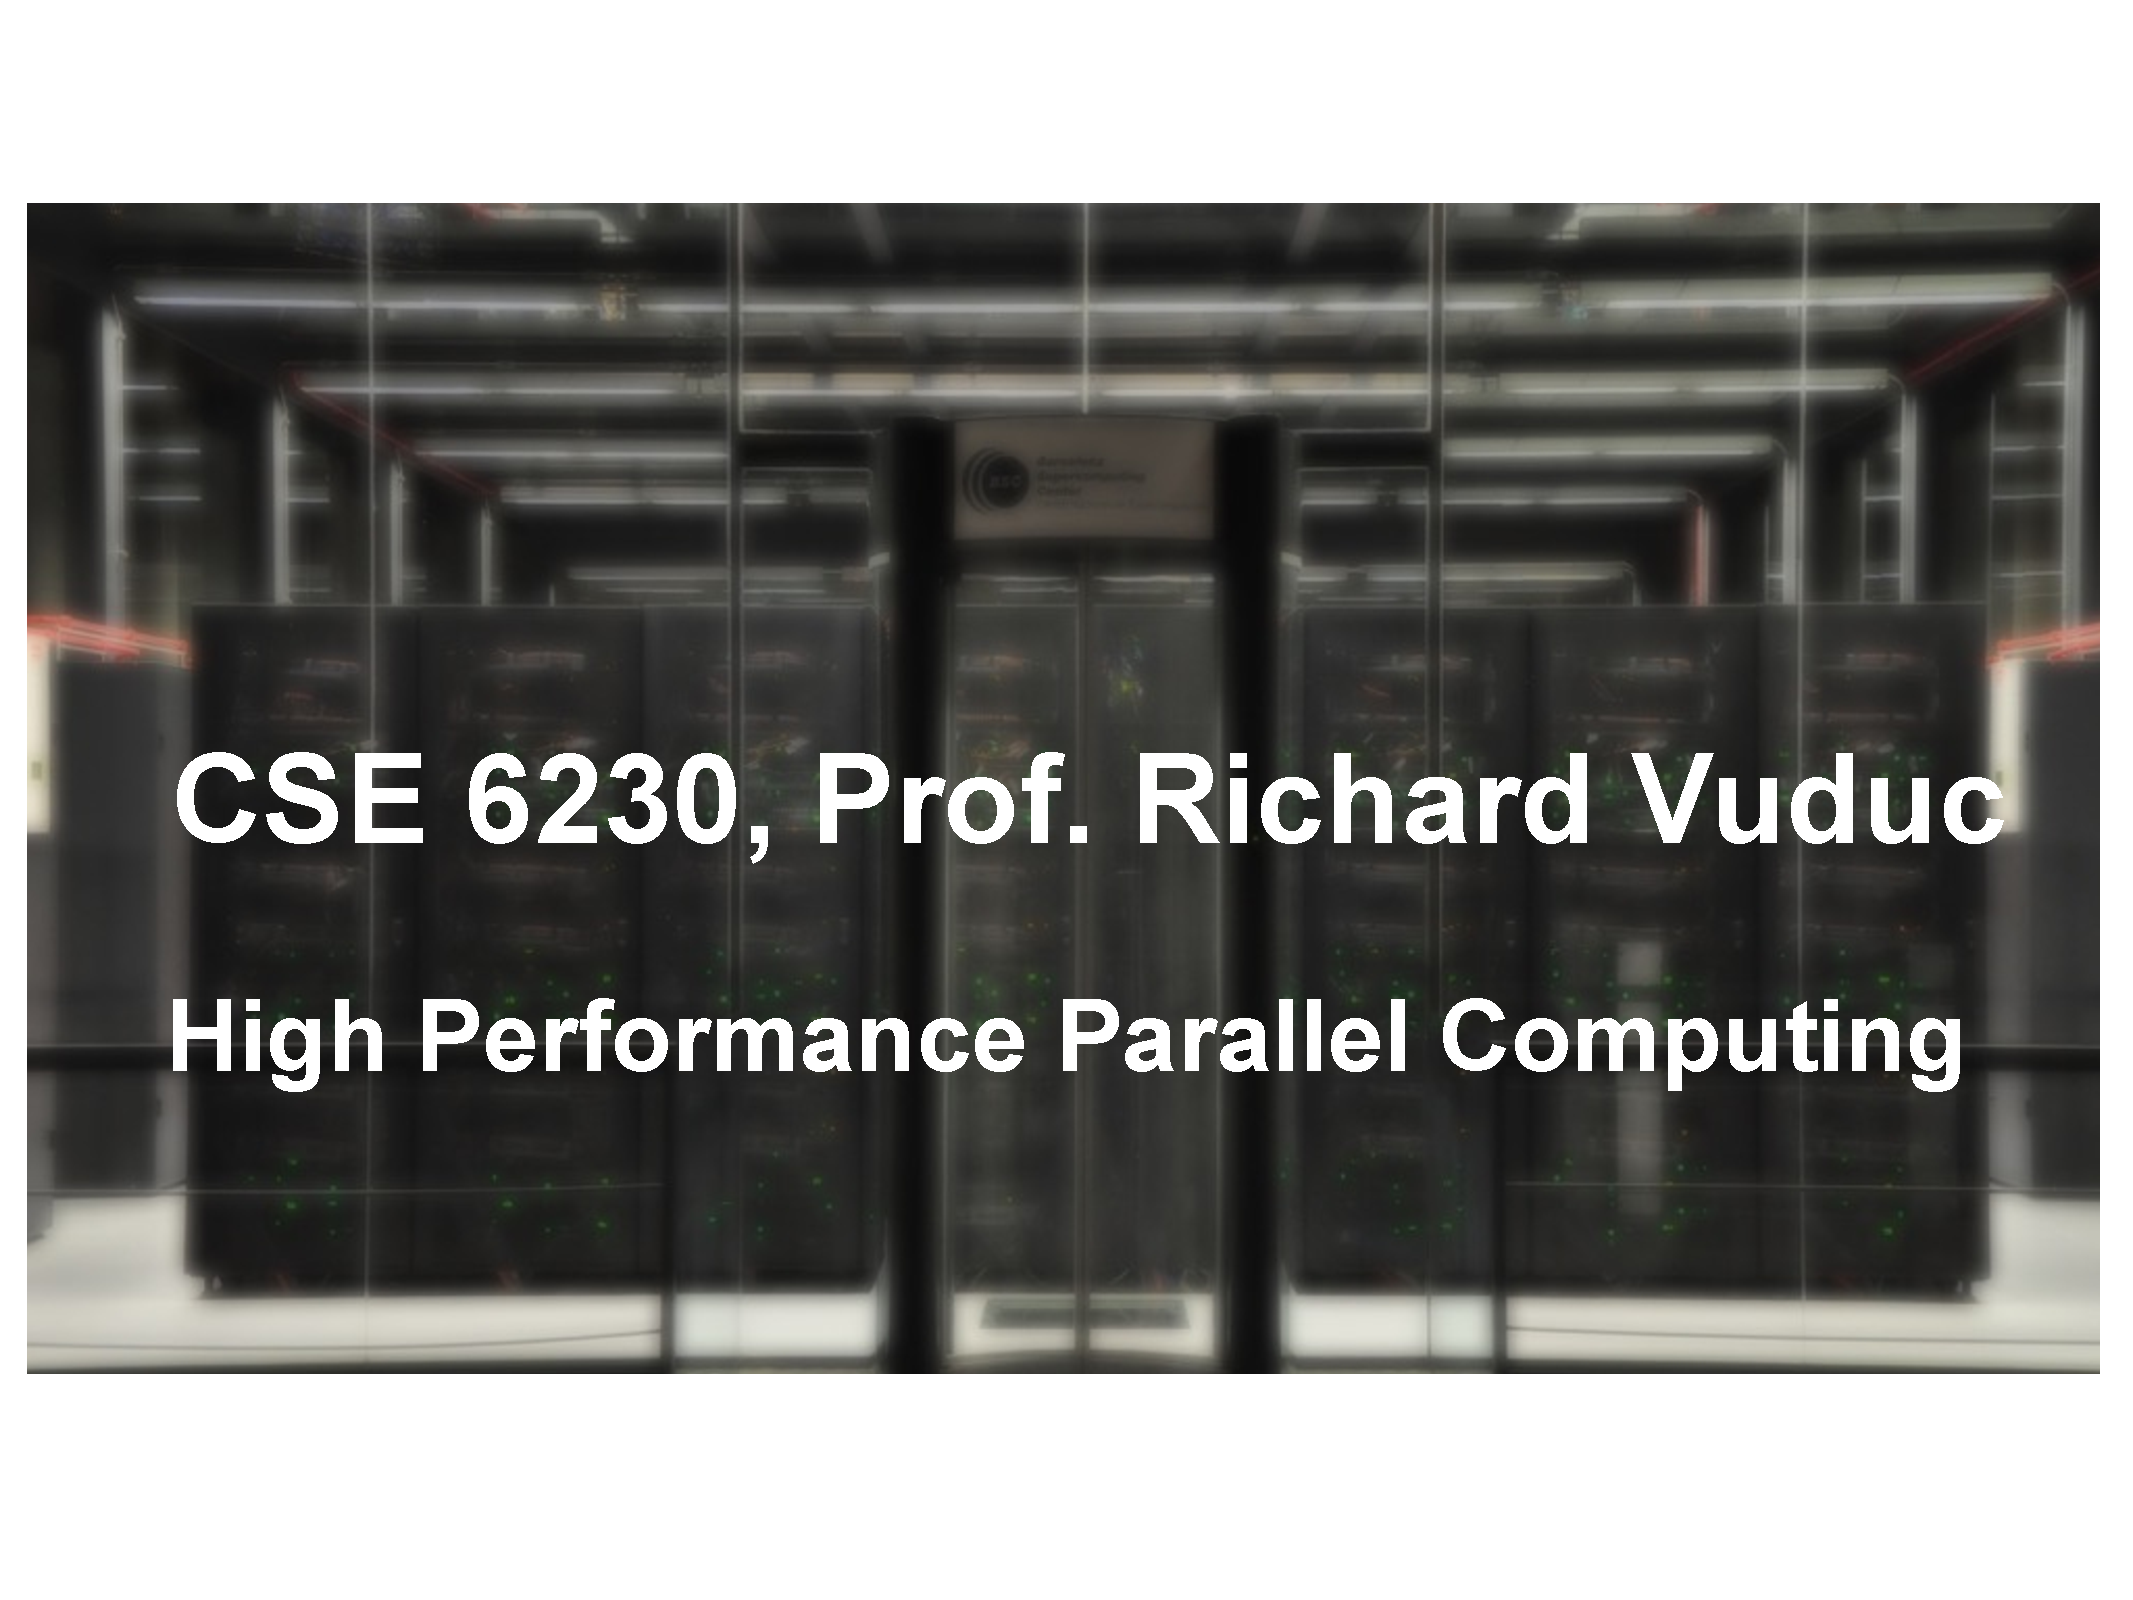
\includegraphics[width=20cm]{logo.pdf}\\
\end{minipage}

\vspace{0.8cm} % A bit of extra whitespace between the header and poster content

%----------------------------------------------------------------------------------------

\begin{multicols}{2} % This is how many columns your poster will be broken into, a portrait poster is generally split into 2 columns

%----------------------------------------------------------------------------------------
%	INTRODUCTION
%----------------------------------------------------------------------------------------

\color{DarkRed} 
\section*{Abstract}
\color{Black} 
%Error correction of short NGS reads is an important component of genome remapping software programs, given huge length of human DNA (of the order of billion). We have picked a state of the art CUDA-EC\cite{shi2010parallel} GPU implementation as the baseline error correction software to improve, for this project. 
%It builds a spectrum of substrings (or k-mers) that occur frequently in the datasets using a bloom filter. The spectrum thus constructed, is then used to correct each read in the dataset.

\emph{We propose a modified parallel implementation for the state of the art error correction software CUDA-EC\cite{shi2010parallel}. We reduce the kernel execution time by approximately \textbf{14.81\%}. This was achieved by increasing warp efficiency from \textbf{3.5\% to 67.5\%} and some other code optimization}


%----------------------------------------------------------------------------------------
%	OBJECTIVES
%----------------------------------------------------------------------------------------

% \color{DarkRed} 
% \section*{Main Objectives}
% \color{Black} 

% \begin{enumerate}
% \item \textbf{Identify the bottlenecks} in the CUDA-EC (CUDA Error Correction) code.
% \item \textbf{Optimise} the code in the runtime determining regions.
% \item Extract the metrics to \textbf{measure success}.
% \item \textbf{Perform experimental evaluation} to measure individual improvements of each modification.

% \end{enumerate}

%----------------------------------------------------------------------------------------
%	MATERIALS AND METHODS
%----------------------------------------------------------------------------------------

\color{DarkRed} 
\section*{CUDA-EC Profiling Results}
\color{Black} 

\begin{enumerate}
\item \textbf{Single GPU thread corrects one read}, leads to high warp divergence (Warp Execution Efficiency 3.5\%)
\item \textbf{No use of shared memory}. extensive use of local memory instead
\item \textbf{High register usage per block}. limits kernel's ability to fully utilize the GPU
\end{enumerate}

%----------------------------------------------------------------------------------------
%	Bloom Filter
%----------------------------------------------------------------------------------------

\color{DarkRed} 
\section*{Improving Bloom Filter's Access throughput}
\color{Black} 
CUDA-EC utilizes bloom filter, a space-efficient probabilistic data structure to hash the frequently occurring k-mers. We tried changing the bloom filter design to make it more cache efficient.
\begin{minipage}{.235\textwidth}
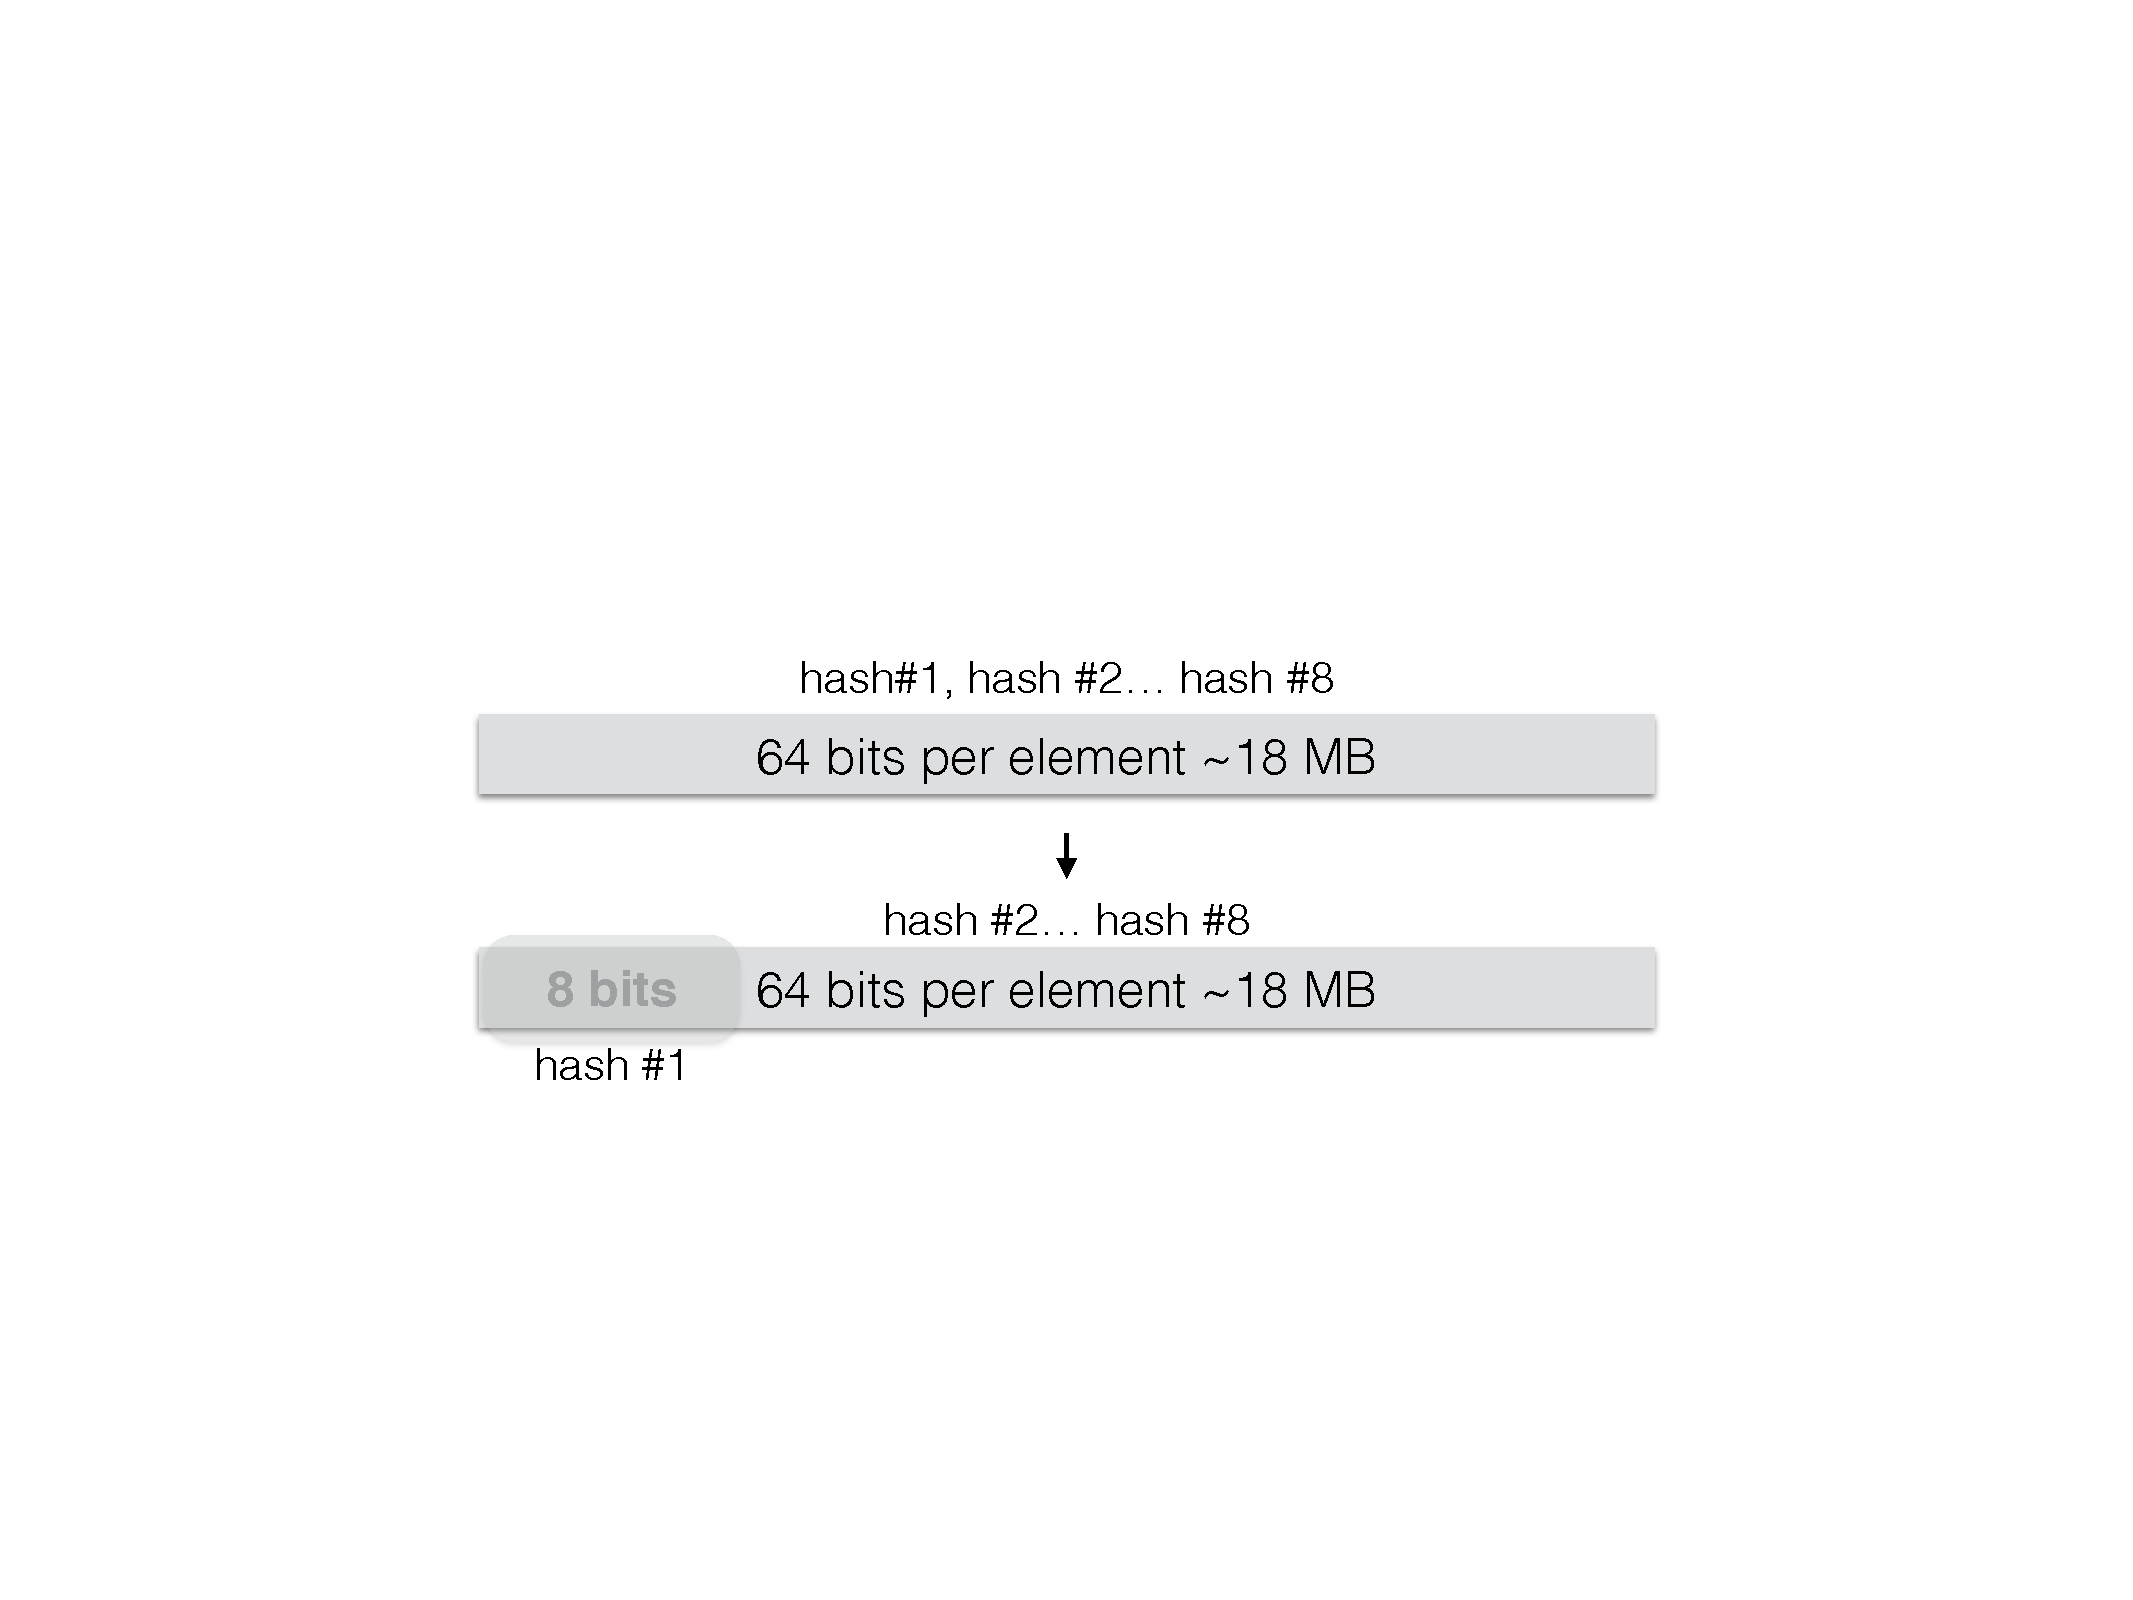
\includegraphics[width=\textwidth]{Hash_Change.pdf}
\end{minipage}
\begin{minipage}{0.235\textwidth}
\begin{center}\vspace{1cm}
\small
\begin{tabular}{l l l}
\toprule
    \bf{Metric}					& \bf{Value (Before)} & \bf{Value (After)}\\
\midrule
    Time 	& 5.73 sec  & 6.16 sec\\
    Texture L2 hit rate 		& 1.96\%  & 14.45\%  \\
    L2 texture throughput		& 2.76 GB/s & 6.29 GB/s\\
    Total texture accesses		& 68,381,701 & 91,551,531\\
\bottomrule
\end{tabular}
\end{center}\vspace{1cm}


\end{minipage}
\vspace{1cm}

%----------------------------------------------------------------------------------------
%	Techniques used 
%----------------------------------------------------------------------------------------

\color{DarkRed} 
\section*{Algorithm and Implementation Details}
\color{Black} 

\begin{enumerate}
\item \textbf{Improving warp divergence:} Restructured the code by having single read processed by one warp
\item \textbf{Using shared memory:} Using selected underlying buffers in shared memory instead of local memory
\item \textbf{Other optimization} 
	\begin{enumerate}
    	\item Loop unrolling
        \item Reducing register count by removing unnecessary variables as well as correcting the scope of some variables
        \item Removing unnecessary copying of reads, simplifying branches
    \end{enumerate}
\end{enumerate}


\begin{minipage}{.235\textwidth}
\small
\begin{algorithm}[H]
	\color{Crimson} %REMOVE_BEGIN
	Allocate vote[] \tcp*{In local memory}
    \color{Black} %REMOVE_END
 	\While{read chunk $\ne$ Empty}
    {
       	\color{Crimson} %REMOVE_BEGIN
        \tcc{Access to read for this thread $tid$}
		$current\_read \gets global\_mem\_all\_reads[tid]$\;
        \color{Black} %REMOVE_END
        \While{$current\_read\_correction\_ongoing$}
        {
            \For{Every $tmpTuple$ k-mer in $current\_read$} 
            {
                \If{$tmpTuple$ is not solid i.e. rare} 
                {
                \color{Crimson} %REMOVE_BEGIN
                    \For{Each character position $i$ in $tmpTuple$} 
                    {
						\color{Black} %REMOVE_END
                        \For{$newtmpTuple \gets$  mutate $i$ with other nucleotides $m:(0\dots3)$}{
                            \If{$newtmpTuple$ is solid}
                            {
                                Update $vote[i][m] += 1$
                            }
                        }
                    }
                }
            }
            \color{Crimson} %REMOVE_BEGIN
            \If{all $tmpTuple$ were solid}
            {
            	\color{Black} %REMOVE_END
            	$current\_read\_correction\_ongoing \gets $FALSE
            }
            \color{Crimson} %REMOVE_BEGIN
            \tcc{Sequential iteration over $vote[][]$ to find maximum $maxVote=vote[p][q]$}
            \color{Black} %REMOVE_END
            \tcc{Update $current\_read[p]$ = Nucleotide[q]}
        }
 	}
\caption{Original CUDA-EC algorithm}
\end{algorithm}
\end{minipage}
\begin{minipage}{0.235\textwidth}
\small
\begin{algorithm}[H]
	\color{DarkGreen} %NEW_BEGIN
	Allocate vote[] 	\tcp*{In shared memory}
    \color{Black} %NEW_END
 	\While{read chunk $\ne$ Empty}
    {
        \color{DarkGreen} %NEW_BEGIN
        \tcc{Access to read for this warp $tid$}
        \tcc{Threads in warp load read to shared mem from global}
		$current\_read \gets shared\_mem\_all\_reads[warp\_id]$\;
        \color{Black} %NEW_END
        \While{$current\_read\_correction\_ongoing$}
        {
            \For{Every $tmpTuple$ k-mer in $current\_read$} 
            {
                \If{$tmpTuple$ is not solid i.e. rare} 
                {
                	\color{DarkGreen} %NEW_BEGIN
                    \For{Each character position $i=0$ in $tmpTuple$; i+=WARPSIZE} 
                    {
                    	\color{Black} %NEW_END
                        \For{$newtmpTuple \gets$  mutate $i$ with other nucleotides $m:(0\dots3)$}{
                            \If{$newtmpTuple$ is solid}
                            {
                                Update $vote[i][m] += 1$\;
                                tmpTupleUnChanged = false\;
                            }
                        }
                    }
                }
            }
            \color{DarkGreen} %NEW_BEGIN
            \If{\_\_all(tmpTupleUnChanged)}
            {
            	\color{Black} %NEW_END
            	$current\_read\_correction\_ongoing \gets $FALSE
            }
            \color{DarkGreen} %NEW_BEGIN
            \tcc{REDUCTION within warp for $vote[][]$ to find maximum $maxVote=vote[p][q]$}
            \color{Black} %NEW_END
            \tcc{Update $current\_read[p]$ = Nucleotide[q]}
        }
 	}
\caption{New CUDA-EC execution flow}
\end{algorithm}
\end{minipage}
\vspace{1cm}

%----------------------------------------------------------------------------------------
%	RESULTS 
%----------------------------------------------------------------------------------------
\color{DarkRed} 
\section*{Results}
\color{Black} 

\vspace*{-2cm}
\begin{center}\vspace{1cm}
\begin{tabular}{l l l}
\toprule
    \bf{Metric}					& \bf{Value (OLD)} & \bf{Value (NEW)}\\
 \midrule
    Warp execution efficiency 	& 3.5\%  & 67.5\%\\
    L1/Shared bandwidth 		& 57.6 GB/s & 146.9 GB/s  \\
    L2 bandwidth				& 7.5 GB/s & 40.6 GB/s\\
    Device memory bandwidth		& 2.0 GB/s (Limit: 208 GB/s) & 37.75 GB/s\\
    Shared memory usage			& 0 bytes & 1.95 KB\\
    Register usage				& 85 per thread & 56 per thread\\
    Occupancy					& 24.6\% & 47.1\%\\
\bottomrule
\end{tabular}
\captionof{table}{Profiling results of original code computed on Kepler K20m GPU}
\end{center}\vspace{1cm}



\begin{minipage}{.235\textwidth}
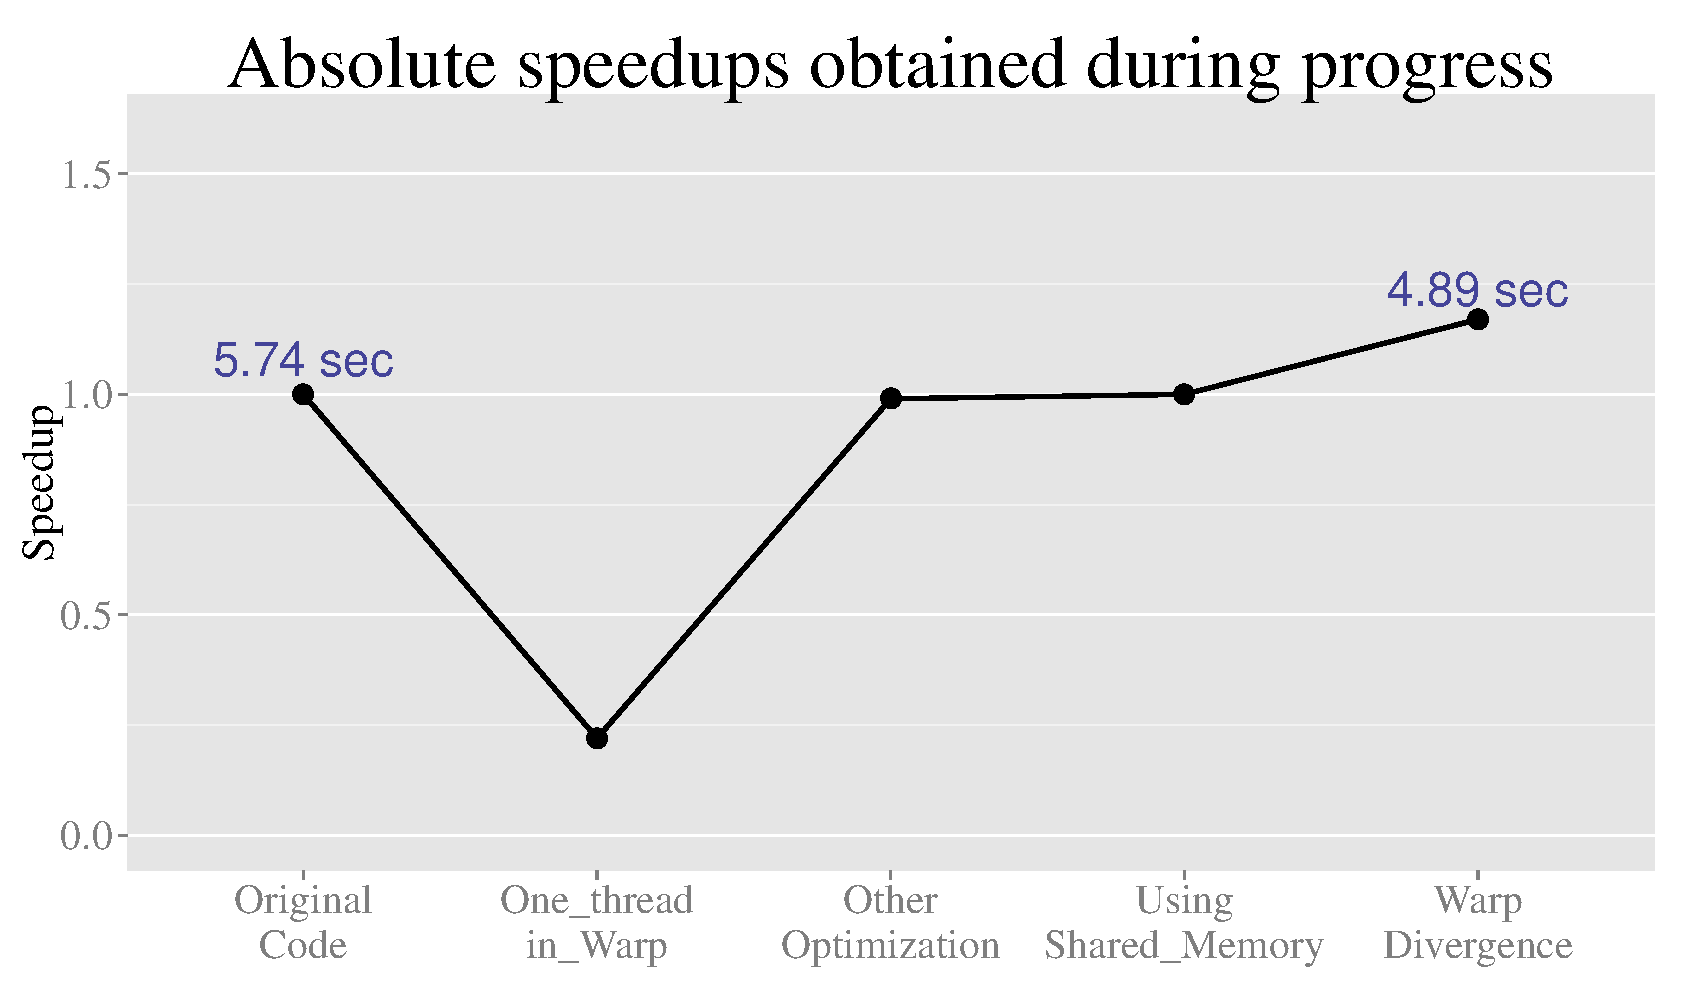
\includegraphics[width=\textwidth]{speedup.pdf}
\end{minipage}
\begin{minipage}{0.235\textwidth}
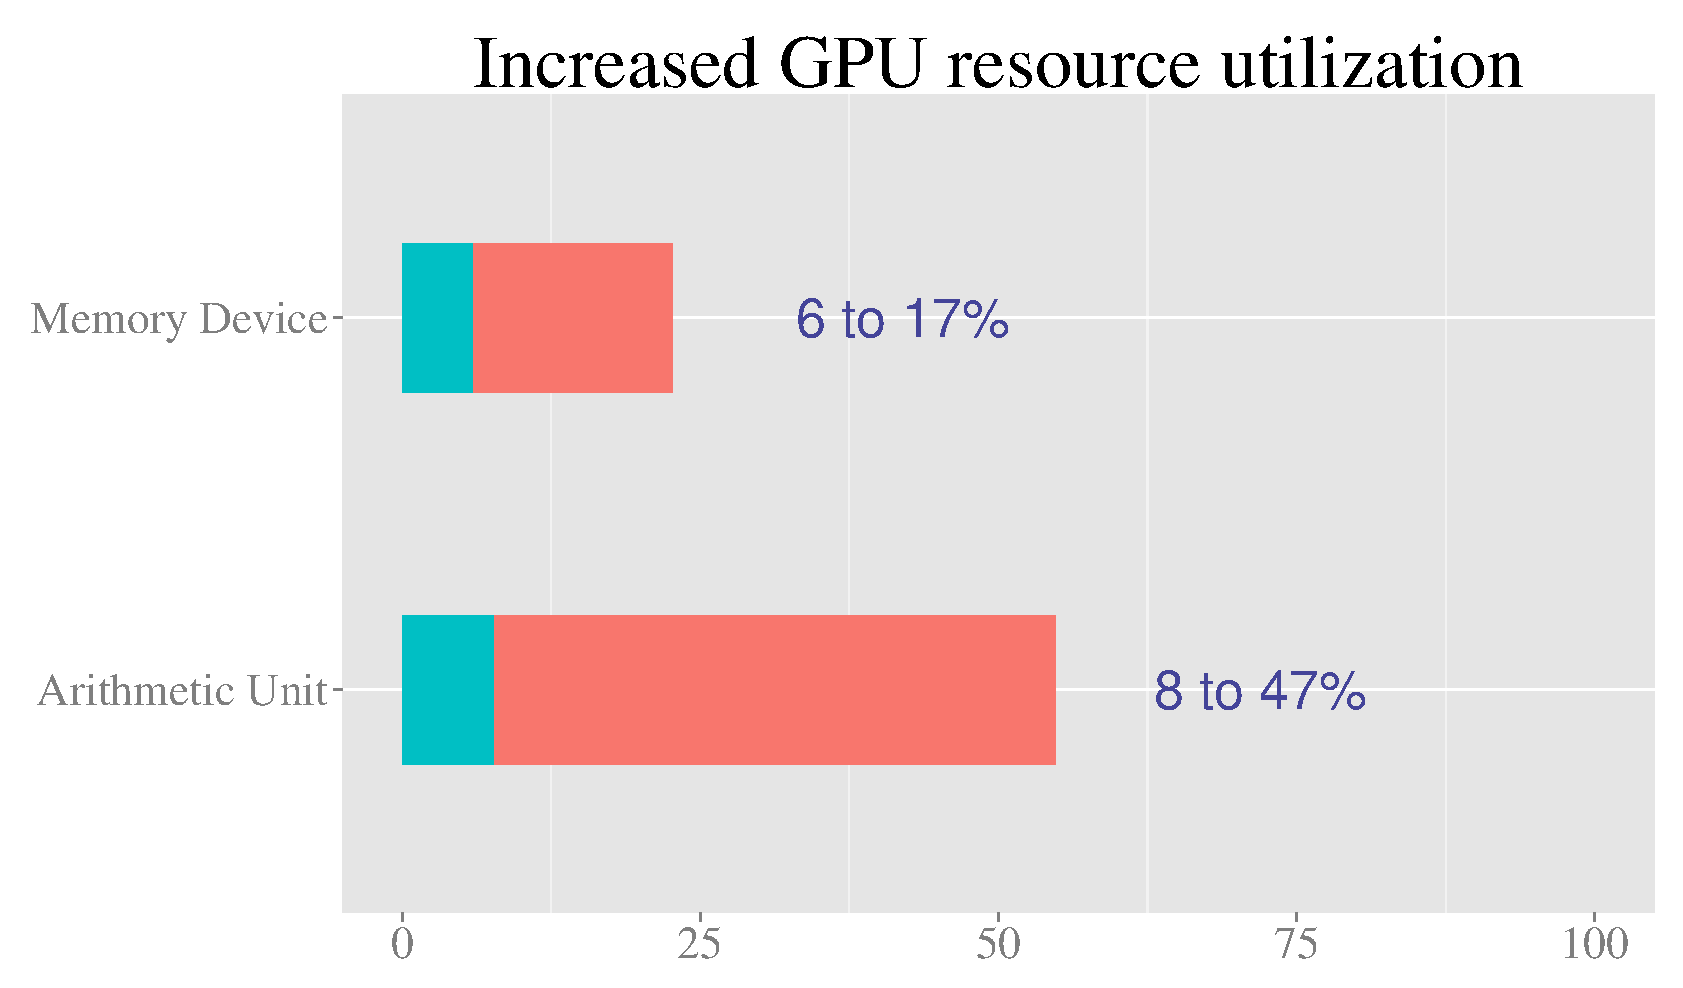
\includegraphics[width=\textwidth]{util.pdf}
\end{minipage}
\vspace{1cm}


%----------------------------------------------------------------------------------------
%	CONCLUSIONS
%----------------------------------------------------------------------------------------

%\color{SaddleBrown} % SaddleBrown color for the conclusions to make them stand out
\color{DarkRed} 
\section*{Conclusions}
\color{Black} 


\begin{itemize}
\item Improved runtime by \textbf{approximately 15\%} without changing output
\item \textbf{Compute and latency bound} algorithm as it performs heavy arithmetic with the available data
\item Showed that \textbf{multiple-threads-one-read} model has enough instruction parallelism to exploit on GPU (classical model is one-thread one-read)
\end{itemize}

%\color{DarkSlateGray} % Set the color back to DarkSlateGray for the rest of the content

%----------------------------------------------------------------------------------------
%	FORTHCOMING RESEARCH
%----------------------------------------------------------------------------------------
\color{DarkRed} 
\section*{Future work}
\color{Black} 

\begin{itemize}
\item Using newly introduced instruction like \textit{shuffle} to carry out reduction operations and communication within a warp
\item Making the software work on large reads and data sets (CUDA-EC itself is not scalable for large reads)
%\item Implementing the algorithm from scratch using latest version of CUDA without constraints such as getting precisely same output data as the original code
\item Rethinking the complete implementation having similar or better accuracy than CUDA-EC.
\end{itemize}

%----------------------------------------------------------------------------------------
%	REFERENCES
%----------------------------------------------------------------------------------------
\color{DarkRed}
\begin{thebibliography}{1}
\color{Black}
  \bibitem{shi2010parallel} Haixiang Shi, Bertil Schmidt, Weiguo Liu, and Wolfgang Muller Wittig. A parallel algorithm for error correction in high-throughput short-read data on cuda-enabled graphics hardware. \em{Journal of Computational Biology}, 17(4):603–615, 2010.
  \end{thebibliography}
  
%\nocite{*} % Print all references regardless of whether they were cited in the poster or not
% \bibliographystyle{plain} % Plain referencing style
% \bibliography{sample} % Use the example bibliography file sample.bib

%----------------------------------------------------------------------------------------
%	ACKNOWLEDGEMENTS
%----------------------------------------------------------------------------------------
\color{DarkRed} 
\section*{Acknowledgements}
\color{Black}

We thank Nagakishore Jammula, senior PhD student at Georgia Tech for his inputs on this problem and allowing us to use CyEnce cluster.

%----------------------------------------------------------------------------------------

\end{multicols}
\end{document}